% %äöüß
%
\chapter{Fundamentals of Organic Semiconductors}\label{chap:Theo}
\addcontentsline{lof}{chapter}{\thechapter\hspace*{1ex} %
Fundamentals of Organic Semiconductors}

%
\intro{In this chapter, the basics of \SC physics are summarized, as they are required for understanding the results presented in this work. Initially the key properties of conventional (inorganic) \SCs (CSCs) are considered. In a second step, organic \SCs (OSCs) are introduced and differences to conventional \SCs are outlined. Finally, the Seebeck effect is discussed and correlations to \SC properties are derived.
}

\newpage

\section{Conventional Semiconductors}\label{sec:TheoConventionalSemiconductors}
This section introduces the fundamentals of \CSCs, in particular the differences between intrinsic and doped \SCs are highlighted. More detailed information can be found in textbooks\cite{Sze,Thuselt,EnderleinSchenk}.
%
\subsection{Intrinsic Semiconductors}\label{sec:Theo-inorg-Bandstructure}%
A \SC (SC) is called intrinsic if it is pure and free of impurities.
A conventional inorganic \SC material, like silicon (Si) or gallium arsenide (GaAs), consists of covalently bound atoms forming a crystalline lattice structure. The discrete energy levels of a single atom are affected by the interaction of the periodically arranged neighboring atoms and a band structure of allowed and forbidden energy eigenstates for electrons is formed.

The population of electrons in the bands depends on the temperature \T. Semiconductors have the special property that at $\T\rightarrow\K{0}$ every band is either completely occupied or empty. Occupied bands are those lying deepest in energy and the highest occupied band is called valence band, whereas the lowest unoccupied band is called conduction band.
The second important property of \SCs is the presence of a forbidden energetic region between the occupied and the empty bands. As only incompletely filled bands can contribute to transport, at $T\rightarrow\K{0}$ charge transport is impossible (unless the material is illuminated or charges are injected).

\begin{wrapfigure}[7]{r}[6.5mm]{22mm}%
{\vspace*{-1.4em}\includegraphics{draw/egap.pdf}}%
\end{wrapfigure}%
In the following, the lowest allowed energy of the conduction band will be called the \EcLong \Ec and the highest allowed energy of the valence band the \EvLong \Ev. The energetic gap between conduction and valence band and hence the difference between \Ev and \Ec is called bandgap \Egap, being a key property of a \SC and is usually in the range of \SIrange{0.5}{2}{\electronvolt}. At room temperature, the typical \SCs Si and GaAS have bandgaps of $1.12$ and \eV{1.42}\cite{Sze}, respectively.

With increasing temperature, an increasing number of electrons from the valence band reaches the conduction band due to their thermal energy, leaving unoccupied states in the valence band, the so-called holes, behind. Holes can be described in a similar manner to electrons and in the following, the indices ``e'' and ``h'' will are used for addressing parameters of electrons and holes, respectively.
%
The \neLong in the conduction band \ne depends on the density of available states $\dos(E)$ in the conduction band and the occupation probability distribution $f(E,T)$, which accounts for the temperature:
\begin{align}
\ne=\int_{-\infty}^\infty \dos(E) \cdot f(E,T) ~ dE
\label{eq:CCD-basic-integral}
\PUNKT
\intertext{Its energy-resolved derivative is called the differential electron density $\n'(E)$:}
\ne'(E)=\dos(E) \cdot f(E,T)
\label{eq:CCD-basic-integral-diff}
\PUNKT
\end{align}
Electrons are fermions\entdecker[Fermi1926]{Enrico Fermi}{Italian}{1901--1954} and therefore each state can only be occupied by one particle. Hence, the occupation probability $f$ is given by the \fFDLong (compare \figref{sim_Fermi-vs-Boltzmann}\,(a)):
\begin{equation} \label{eq:fFD}
\fFD(E,T) = \frac{1}{1+\exp{\frac{E-\Ef}{\kT}}}
\PUNKT
\end{equation}
Here, \kB is Boltzmann's\entdecker{Ludwig Eduard Boltzmann}{Austrian}{1844--1906} constant and at \T[25] the product $\kT=\meV{25.7}$. %0.025692751856473 eV
\Ef is the electro-chemical potential which is temperature-dependent as well. For $\T\to\K{0}$, the \fFDLong becomes a step function and the occupation probability is zero for all states with an energy above the chemical potential ($f_\text{FD}(E,T)=0$ for $E>\Ef$ at $T\to\K{0}$). The highest occupied energy state at \K{0} is called Fermi \emph{energy}. %$\Ef^0$
At higher temperature, the chemical potential is called Fermi \emph{level} and is temperature-dependent. In the following, only the term Fermi level will be used, since all temperatures discussed are well above \K{0}. The Fermi level is the energy correlated to an occupation probability of $50\,\%$ $(\fFD(\Ef,T)=0.5)$. In case of intrinsic \SCs discussed so far, the value of \Ef is close to the middle of the bandgap, compare \eqnref{EfPosIntrinsic} below.

The \fFDLong can be approximated by the \fBLong for $E-\Ef\gg\kT$
\begin{equation}\label{eq:fB}
\fB(E,T)
  = \exp{-\frac{E-\Ef}{\kT}}
\PUNKT
\end{equation}
\Figref{sim_Fermi-vs-Boltzmann}\,(b) compares the two functions and it can be seen that at $E=\Ef$ the value of $\fB(E)$ is twice the value of $\fFD(E)$. At higher energies the error is strongly decreasing \eg already at $E=\Ef+3\,\kT$, the overestimation is as small as $\approx 5\,\%$. A general expression for the overestimation of $\fFD(E)$ by using $\fB(E)$ can be written as
\begin{equation}
\frac{\fFD(E)}{\fB(E)} - 1 = \exp{-\frac{E-\Ef}{\kT}} = \fB(E)
\KOMMA
\end{equation}
which interestingly is identical to the \fBLong itself.

\cBild[t]
{sim_Fermi-vs-Boltzmann}
{Fermi-Dirac and Boltzmann distribution functions}
{(a) \fFDLong $\fFD(E)$ for the occupation probability at \T[25], \K{0} and \grad{100}. (b) Comparison of Fermi-Dirac $\fFD(E)$ and \fBLong $\fB(E)$ for $\T[25]$ ($\kT=\meV{25.7}$).
} % 25C = 25.7meV

The \dosLong of an intrinsic \CSC is zero in the energy gap between valence and conduction band and non-zero in the bands. Close to the minimum of the conduction band it can be approximated by a square root proportionality to the energy above \Ec\cite{Sze} :
\begin{align} \label{eq:DOS-inorg-prop-sqrt}
 \dos(E) &\propto \sqrt{E-\Ec} & \text{for } E>\Ec \PUNKT
\end{align}
% \Eqnref{CCD-basic-integral} for the charge carrier density \ne can therefore be written
% \begin{equation}
% \ne \propto \int_{\Ec}^\infty \sqrt{E-\Ec} \cdot \fDF(E,T) dE
% \PUNKT
% \end{equation}
Using this \dosLong and the Boltzmann approximation for the \fFDLong \fFD, \eqnref{CCD-basic-integral} can be solved analytically to
\begin{align}
\ne&=\Nc\exp{-\frac{\Ec-\Ef}{\kT}}
\label{eq:ne-InOrg-via-Boltzmann}
\PUNKT
\intertext{Analogously to electrons, the \nhLong \nh in the valence band can be derived, resulting in}
  \nh&=\Nv\exp{-\frac{\Ef-\Ev}{\kT}}
\label{eq:nh-InOrg-via-Boltzmann}
\PUNKT
\end{align}
The prefactors \Nc and \Nv are the so-called effective \dosLong in the conduction and valence band, both being proportional to $(\kT)^{3/2}$ and of the unit \si{\per\centi\meter\cubed}.
%when again using the Boltzmann approximation.

The above equations are only valid in thermal equilibrium and have to be modified if an external bias voltage or illumination is applied to the system. Exemplary, the absorption of a photon would lead to an increase of both, \ne and \nh, making it impossible to describe the system with one Fermi level. Instead, separate quasi-Fermi levels for electrons and holes have to be introduced if thermal relaxation inside the bands is much faster than relaxation from band to band.

In an uncharged and undisturbed intrinsic \SC at a given temperature, the number of electrons in the conduction band equals the number of holes in the valence band (neutrality condition). This density is called the intrinsic charge carrier density \ni
\begin{equation} %\label{eq:NeuralityConditionIntr}
 \ne = \nh = \ni
\PUNKT
\end{equation}
It is important to note that the square of $n_\text{i}$
\begin{equation} \label{eq:LawOfMassAction}
 \ni^2 = \ne \cdot \nh = \Nc\Nv\exp{-\frac{\Egap}{\kT}}
\KOMMA
\end{equation}
is independent of the Fermi level \Ef and can be calculated from \Nv, \Nc, and the bandgap \Egap. Equation~\eqref{LawOfMassAction} is the law of mass action, known from basic chemistry. % http://en.wikipedia.org/wiki/Mass_action_law_(electronics)

\subsection{Doped Semiconductors} \label{sec:TheoDopedSCs}% Doping ?
In order to increase the number of free charge carriers \neh of a \SC, suitable impurities of other elements can be introduced.
In a so-called doped \SC, some of the atoms in the lattice structure are replaced by atoms of a different material, having one valence electron more or one valence electron less than the host element. These impurities are called dopants.

In case of a dopant with one additional valence electron, this electron is only weakly bound inside the lattice of the host material, as no partner for a covalent bond is available. Hence, only little thermal energy is needed for this electron to reach the conduction band and thus to increase the \neLong \ne. Such dopants are called donors or n-dopants as they donate their negatively charged valence electron to the host material.

The same principle works in an analogous manner for dopant atoms that have one valence electron less than the host.
These dopants are called acceptors or p-dopants since a valence electron of the surrounding host atoms is taken and a positively charged hole is created on the host.

Silicon, for example, is typically n-doped using phosphorus (P) as donor or p-doped using boron (B) as acceptor with typical dopant concentrations in the range of a few parts per million (ppm).

In the following, \Nd and \Na are the absolute values of the dopant concentration of donors and acceptors in the host material, usually given in the unit \si{\per\centi\meter\cubed}.
The energy levels of the dopants are located in the bandgap of the host. While the donor level \Ed is near the conduction band (below \Ec), the acceptor level \Ea is near the valence band (above \Ev).

\subsubsection{Ionization of Dopants}
Thermal energy is needed for the ionization of dopants and thus generation of free charges for the conduction or valence band. Two classes of dopants can be distinguished: dopants with either a \emph{deep} or a \emph{shallow} level with respect to the host material. Shallow dopants have an energy level than close to the band edge that thermal energy is sufficient to ionize (most of) them. Deep dopants on the other hand, have energy levels several \kT away from the band edge, so that ionization is less probable.
Generally, the density of ionized donors \Ndi and ionized acceptors \Nai are\cite{Shockley}
\begin{align}
\Ndi &= \Nd \left(
1-
\frac
{1}
{1 + \frac{1}{\gd} \exp{\Ed-\Ef}{\kT}}
\right)
\label{eq:DefNdi}
\\
\Nai &=\Na
\left(
\frac
{1}
{1 + \ga \exp{\Ea-\Ef}{\kT}} \right)
\label{eq:DefNai}
\KOMMA
\end{align}
with \ga and \gd being the ground state degeneracy of the donor and acceptor levels. Typically the degeneracy of these levels is $g=2$ as each level can be occupied by two electrons of opposite spin $(\pm\sfrac{1}{2})$. Additional degeneracy can be introduced by the host material. For Si and GaAs, the valence band is twofold degenerate and thus they have two hole levels each being twofold spin degenerate, leading to a value of $\ga=4$ in these materials.
The temperature regime, where the thermal energy is sufficient to ionize almost all dopants ($\Ndi\approx\Nd$ and $\Nai\approx\Na$) is called the saturation range.
%
The ratio of the \nLong \neh to the density of dopants can be defined as doping efficiency \DopEff (for $\Nd\gg\ni$):
\begin{align}
 \DopEff &= \frac{\ne}{\Nd} \quad \text{or}\quad \DopEff = \frac{\nh}{\Na}
\label{eq:DepEff-inorg}
\PUNKT
\end{align}

The law of mass action ($\ni^2 = \ne \cdot \nh$, \eqnref{LawOfMassAction}) is valid for doped \SCs as well. In contrast to intrinsic SCs, for doped SCs the \neLong in the conduction band \ne does not equal the \nhLong in the valence band \nh. Hence, the neutrality condition for doped SCs has to include the ionized dopants as well:
\begin{align}
\ne + \Nai &= \nh + \Ndi
\label{eq:NeuralityCondition} \\
\begin{split}
\Rightarrow
\Nc\exp{-\frac{\Ec-\Ef}{\kT}}
%
&+
%
\Na
\left(
\frac
{1}
{1 + \ga \exp{\Ea-\Ef}{\kT}} \right)
\\
=
%
\Nv\exp{-\frac{\Ef-\Ev}{\kT}}
&+
%
\Nd \left(
1-
\frac
{1}
{1 + \frac{1}{\gd} \exp{\Ed-\Ef}{\kT}}
\right)
\label{eq:NeuralityConditionLong}
\KOMMA
\end{split}
\end{align}
(Boltzmann approximation used).

If, for example in an n-doped SC, only donors and no acceptors ($\Na=0$, $\Nd>0$) are present, the neutrality condition \eqref{NeuralityCondition} and the law of mass action \eqref{LawOfMassAction} can be used to derive an expression for the \neLong in the condition band \ne\cite{Thuselt}:
\begin{align}
 \ne &= \nh + \Ndi \quad \text{and} \quad \nh = \frac{\ni^2}{\ne} \quad \Rightarrow \quad \ne^2 - \ne \Ndi-\ni^2 = 0 \nonumber \\
 \ne &=\frac{\Ndi}{2} + \sqrt{\left(\frac{\Ndi}{2}\right)^2 + \ni^2}
\PUNKT
\end{align}
This clearly shows the two sources for the \neLong in the conduction band: the excited electrons from the valence band and those from the ionized donors. An analogous trend can be found for acceptor-only doping and \nh.

\subsubsection{Fermi Level Position}\label{sec:FermiLevelPosition}\label{sec:TheoDegenerateDoping}
For an intrinsic \SC, the \EfLong \Ef is located close to the middle of the bandgap:
\begin{equation}
 \Ef = \frac{\Ec+\Ev}{2} + \frac{\kT}{2}\cdot \ln \left(\frac{\Nv}{\Nc}\right)
\PUNKT
\label{eq:EfPosIntrinsic}
\end{equation}
Introducing dopants leads to a shift of \Ef. In case of n-doping, the Fermi level moves towards the conduction band, whereas for p-doping, it moves towards the valence band.
By solving the neutrality condition \eqref{NeuralityConditionLong}, the value of \Ef can be calculated, keeping in mind that all four terms (\ne, \nh, \Ndi, \Nai) depend on \Ef.

In case of shallow dopants or at elevated temperatures, when most dopants are ionized, the position of \Ef is given by:
\begin{align}
 \Ef &= \Ec - \frac{\kT}{2}\cdot \ln \left(\frac{\Nc}{\Nd}\right) & \text{for n-doping} \\
 \Ef &= \Ev + \frac{\kT}{2}\cdot \ln \left(\frac{\Nv}{\Na}\right) & \text{for p-doping}
%\PUNKT hier sieht ein Punkt häßlich aus
\end{align}

\begin{figure}[b]
\centering%
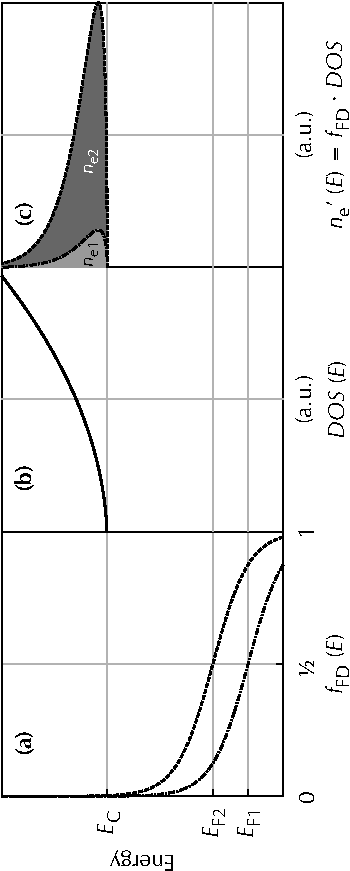
\includegraphics[angle=-90]{plot/sim_Fermi-DOS-n-inorg}%
\setcapwidth[c]{\tmCapWidth}%
\caption
[Influence of \Ef on $\fFD(E)$ and \ne]
{Influence of Fermi level \Ef on \fFDLong $\fFD(E)$ and \neLong \ne for n-doping: (a) $\fFD(E)$ for two different positions of \Ef below the \EcLong \Ec, $\Ef${}$_1=\Ec-\meV{200}$ and $\Ef${}$_2=\Ec-\meV{150}$ (b) \dosLong $\dos(E)$ (c) product of $\fFD(E)$ and $\dos(E)$, displaying the strong influence of \Ef on the \neLong \ne corresponding to the area under the curve.}
\label{fig:sim_Fermi-DOS-n-inorg}
\end{figure}
%
The influence of \Ef on the \fFDLong \fFD and hence on the \neLong \ne, being the integrated product of \fFD and the \dosLong \dos, is displayed in \figref{sim_Fermi-DOS-n-inorg}. It is drawn for the case of n-doping, hence \Ef shifts towards \Ec.
Two \fFDLong{s} with different values of \Ef, corresponding to different doping concentrations, are drawn in part~(a). $\Ef${}$_1$ is chosen to be \meV{200} below \Ec, $\Ef${}$_2$ is \meV{50} larger and hence \meV{150} below \Ec.
In part~(b) of the figure, the \dos is sketched, showing a square root dependency on the energy above the conduction band minimum \Ec, compare \eqnref{DOS-inorg-prop-sqrt}. Finally, the products of \dosLong and the two different Fermi-Dirac distribution functions are drawn in part~(c). These products correspond to the differential \neLong $\ne'(E)$, as shown by \eqnref{CCD-basic-integral-diff}. Therefore, the areas under the curves are the total densities of free electrons $\ne${}$_1$ and $\ne${}$_2$, respectively, compare \eqnrefPage{CCD-basic-integral}.
For the chosen values of $\Ef${}$_1$ and $\Ef${}$_2$, the \neLong $\ne${}$_2$ is 7~times larger than $\ne${}$_1$, which displays the strong influence of the Fermi level position on the \neLong.
An analogous picture can be drawn for p-doping, where \Ef shifts towards the \Ev and increases the \nhLong \nh.

Extremely high doping concentrations result in the Fermi level approaching the band edge. At a difference less than $2\,\kT$, the \SC properties are vanishing and metallic behavior is observed. Furthermore, the Boltzmann approximation for the \fFDLong is not valid for these so-called degenerate \SCs and the equations can only be solved numerically.

\subsection{Charge Carrier Transport}\label{sec:TheoDiffusionCurrent}\label{sec:TheoDriftCurrent}
Free charges (holes in the valence band and electrons in the conduction band) are in constant motion due to their thermal energy. Besides this random thermal movement, an ordered/directed transport is possible under two conditions: Diffusion transport due to a gradient in the \nLong and hence \Ef in the material and drift transport due to the presence of an electrical field. % Both cases are discussed in the following.

% \subsubsection{Diffusion}
Diffusion transport is the thermally driven motion of charges from regions of higher to regions of lower charge carrier concentration. Hence, diffusion transport takes place if a gradient in the \nLong is present in the material.
Fluctuations of the charge carrier concentration can be generated for example by different temperatures in the material (compare \secref{TheoSeePhenomenological}) or by local excess carrier generation.

% \subsubsection{Drift}
Drift transport is the directed motion of charges, driven by the presence of an electric field \EField. Each electron carries one negative elementary electric charge $-e$, whereas a hole (being an unoccupied electron state) carries $+e$.
An electric field leads to a Coulomb%
\entdecker[Coulomb1785a]{Charles Augustin de Coulomb}{French}{1736--1806} 
force accelerating electrons and holes in opposite directions.

The mean drift velocity $v_\text{d}$ of the charges in direction of the force is proportional to the electric field \EField. The proportionality factor of the unit~\si[per=frac]{\centi\meter\squared\per\volt\per\second} is called the mobility \mob and is usually different for electrons and holes:
\begin{align}
 v_\text{d}^\text{e} = \mobe \cdot \EField & & v_\text{d}^\text{h} = \mobh \cdot \EField \label{eq:vdrift}
\PUNKT
\end{align}
In a general case, \eg for non-isotropic materials, the mobility is a tensor and \lasteqn must be read vectorially. The mobility of charges in a \SC depends on many parameters, \eg morphology, \nLong, electric field and temperature. At low temperatures, the mobility is limited by scattering at ionized impurities, due to the low energy and hence low velocity of the charge carriers. Therefore, a decrease in temperature usually leads to a decrease in mobility. At high temperatures on the other hand, the charge carrier motion is disturbed by lattice vibrations, so-called phonons, leading to a decreasing mobility as well. In the temperature region between these two regimes, typically around room temperature, the mobility has a maximum.

% \subsubsection{Conductivity}
As the electric field \EField is defined as the gradient of the electric potential $V$, a field across a material can be generated by applying different electrical potentials to either side of the material.
Applying a voltage~$V$ between two parallel sheet contacts of distance \dc the resulting electric field \EField is
\begin{equation}\label{eq:Efield}
\EField = \frac{dV}{dx} = \frac{V}{\dc}
\PUNKT
\end{equation}

The drift of charges towards the contacts sum up to a current flow $I$ through the material, following Ohm's%
\entdecker[Ohm1827]{Georg Simon Ohm}{German}{1789--1854}
law. In case of a material cross-section $A$, Ohm's law can be written as
\begin{align}
I&=\frac{1}{R}\cdot V = \frac{A \c}{\dc}\cdot V \Rightarrow \c = \frac{I}{V} \cdot \frac{d_\text{c}}{A}
\label{eq:Cond-I-V-geo}
\KOMMA
\end{align}
with the conductivity \c of the material defining its resistance $R=\sfrac{d_\text{c}}{A \, \c}$. The typical unit used for the conductivity of \SCs is $\si{\siemens\per\centi\meter} = \si[per=frac]{\per\ohm\per\centi\meter}$. Applying a voltage~$V$ and measuring the current response $I$, the conductivity of the material can be calculated using \lasteqn.

Instead of the total current $I$, the geometry independent current density $j=\sfrac{I}{A}$ is used to compare different measurements.
The current density can be written as the sum of electron and hole contributions, each being the product of the \nLong and their mean velocity:
\begin{equation}
 j = e \ne v_\text{d}^\text{e} + e \nh v_\text{d}^\text{h}
\PUNKT
\end{equation}
Combining equations \eqref{vdrift}-\lasteq, the conductivity of a \SC can be written as
\begin{equation} \label{eq:Cond-CCD-Mob}
 \c = e \cdot \ne \cdot \mobe  + e \cdot \nh \cdot \mobh
\PUNKT
\end{equation}

